%<dscrpt>Coniques homofocales, sinus et cosinus complexes</dscrpt>
\def\Cos{\textnormal{Cos}}
\def\Sin{\textnormal{Sin}}
Dans ce problème \footnote{d'après un problème de Serge Dupont (\href{http://moduloserge.free.fr/}{http://moduloserge.free.fr/}) } les termes \emph{arc paramétré} et \emph{courbe paramétrée} ont la même signification. Un arc paramétré est dit régulier si et seulement si il est sans point stationnaire.

On désigne par $\mathcal P$ un plan euclidien orienté muni d'un repère orthonormé direct $\mathcal R$. Les coordonnées et les affixes des points du plan sont relatifs à ce repère.\newline
Soient $a$ et $b$ des réels strictement positifs. On définit une hyperbole  $\mathcal H_ {a,b}$ et une ellipse $\mathcal E_{a,b}$ par leurs équations réduites :
\begin{align*}
 \mathcal H_ {a,b} :\qquad \frac{x^2}{a^2} - \frac{y^2}{b^2} = 1 & &
 \mathcal E_{a,b} :\qquad \frac{x^2}{a^2} + \frac{y^2}{b^2} = 1 \text{ pour }a\geq b
\end{align*}
Soient $F$ et $F'$ les points respectivement de coordonnées $(1,0)$ et $(-1,0)$.\newline
On définit les fonctions $\Cos$ et $\Sin$, de $\C$ dans $\C$ par:
$$ \forall z\in \C, \;\Cos\ z = \frac12 \left(e^{iz} + e^{-iz}\right) \qquad 
\Sin\ z = \frac1{2i} \left( e^{iz} - e^{-iz}\right).$$


\begin{enumerate}
\item Soit $Z = \{z \in \C\, | \, \Cos\ z =0\}$ et $I$ un intervalle ouvert.\newline
Soit $\gamma_{1}$ et $\gamma_{2}$ deux fonctions de classe $\mathcal C^1$ définies dans $I$ et à valeurs dans $\C \setminus Z$. On suppose que :
\begin{displaymath}
 \forall t\in I,\; \gamma'_1(t)\neq 0 \text{ et } \gamma'_2(t)\neq 0
\end{displaymath}
On définit des arcs paramétrés $g_1$, $g_2$, $f_1$, $f_2$ par :
\begin{displaymath}
 \forall t\in I ,\;
\left\lbrace 
\begin{aligned}
 g_1(t) &\text{ est le point d'affixe } \gamma_1(t) \\
 g_2(t) &\text{ est le point d'affixe } \gamma_2(t) \\
 f_1(t) &\text{ est le point d'affixe } (\Sin \circ \gamma_1) (t) \\
 f_2(t) &\text{ est le point d'affixe } (\Sin \circ \gamma_2) (t)
\end{aligned}
\right. 
\end{displaymath}

\begin{enumerate}
\item  Déterminer $Z$. 
\item On admet que les fonctions $\Sin \circ \gamma_1$ et $\Cos \circ \gamma_2$ sont $\mathcal C^1$ avec :
\begin{displaymath}
 \forall t\in I, (\Sin \circ \gamma_1)'(t) = \Cos(\gamma_1(t))\gamma_1'(t), (\Sin \circ \gamma_2)'(t) = \Cos(\gamma_2(t))\gamma_2'(t) 
\end{displaymath}
Montrer que les arcs paramétrés $f_1$ et $f_2$ sont réguliers. 
\item On suppose que $\gamma_1(t_0) = \gamma_2(t_0)$ pour un certain $t_0\in I$. Montrer l'\'egalit\'e des angles orient\'es 
\begin{displaymath}
 \widehat{(\overrightarrow{f_{1}}'(t_0),\overrightarrow{f_{2}}'(t_0))} =
 \widehat{(\overrightarrow{g_{1}}'(t_0),\overrightarrow{g_{2}}'(t_0))}\ [2\pi]
\end{displaymath}
 \emph{(On dit que l'application $\Sin$ est conforme.)}
\end{enumerate}

\item \`A quelle condition sur $a$ et $b$ l'hyperbole $\mathcal H_{a,b}$ (respectivement l'ellipse $\mathcal E_{a,b}$) a-t-elle pour foyers $F$ et $F'$ ? 
\item Soit $y_0>0$. Montrer que l'image par $\Sin$ d'une droite d'équation $y=y_0$ est une ellipse de foyers $F$ et $F'$. 
\item Soit $x_0 \in \left]0, \frac{\pi}2\right[$. Montrer que l'image par $\Sin$ de l'ensemble d'équation $x^2 = x_0^2$ est une hyperbole de foyers $F$ et $F'$. 
\item On dit que deux courbes $\Gamma$ et $\Gamma' $ sont orthogonales si en tout point $M \in \Gamma \cap \Gamma'$, les tangentes à $\Gamma$ et $\Gamma'$ sont perpendiculaires.\newline
Montrer qu'une hyperbole et une ellipse de foyers $F$ et $F'$ sont orthogonales.
\end{enumerate}
\begin{figure}[h!]
 \centering
 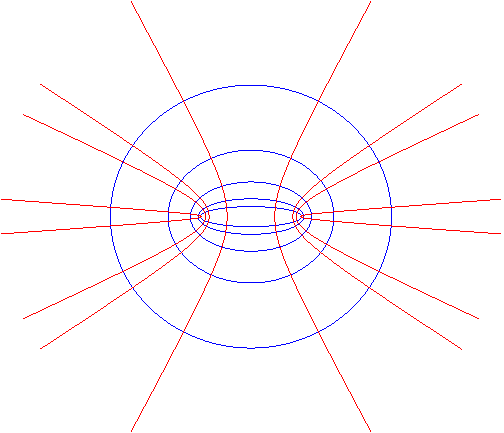
\includegraphics{Esincosc_1.pdf}
 % Esincosc_1.pdf: 0x0 pixel, 0dpi, 0.00x0.00 cm, bb=
 \caption{Hyperboles et ellipses homofocales}
 \label{fig:Esincosc_1}
\end{figure}
